% This file was converted to LaTeX by Writer2LaTeX ver. 1.0.2
% see http://writer2latex.sourceforge.net for more info
\documentclass[12pt]{article} %scrartcl


% bibliographie
%\usepackage[round]{natbib}
\usepackage[natbib=true,backend=bibtex,sorting=nyvt, isbn= false, url=false, doi=false,eprint=false, style=authoryear]{biblatex}
\addbibresource{/home/alain.danet/Dropbox/Shared_TheseAlain/BibTeX/M2-StageM2,/home/alain.danet/Dropbox/Shared_TheseAlain/BibTeX/Thesis}

%accents, language français
\usepackage[utf8]{inputenc}
\usepackage[T1]{fontenc}
\usepackage[english]{babel} %
\usepackage{csquotes}
%\usepackage{xltxtra}


%Image
\usepackage{graphicx}
\usepackage{subcaption}
\usepackage{tikz}
\usetikzlibrary{arrows,shapes}
\graphicspath{{/home/alain.danet/Dropbox/Shared_TheseAlain/Figures/}}

% Font

% Outline numbering
\setcounter{secnumdepth}{0}
% Set interligne
\linespread{1.5}
% Page layout (geometry)
%\geometry{left=2.5cm,right=2.5cm,top=2.5cm,bottom=2.5cm}
% Pages styles
\pagestyle{plain}



% Page de titre
\title{Experiment: Modulation of interaction following functional plant type across grazing et water stress gradients}
\author{\textbf{Alain Danet}}


\date{Octobre 2014}


\begin{document}

\maketitle


\part{Introduction}
The theory of Stress Gradient Hypothesis (SGH) predict basicly a increasing of facilitation importance when stress increase. This hypothesis has been widely tested and stay still in debate because of opposite results. Two of main obstacles are (i) the fact all the species have not the same potential to be facilited and conversely all the species have not the same potentiel to facilitate; (ii) We have not the same assumptions if the "stress" is based on stress (eg water) or disturbance (eg grazing) (sensu Grime) \citep{Maestre2009}.

As \citet{Butterfield2013} suggested, take a functional approach of facilitation will permit us to better understand the context dependance of facilitation. He predicts stress would result in facilitation of competitive species and disturbance would result in facilitation of competitive or stress-tolerator species. So far, we don't know any experimental studies which have explicitly related Grime plant strategies to SGH. On the other hand, some observational studies described plant strategies along grazing gradient \citep{DIAZ2007}. 

\begin{figure}
\begin{center}
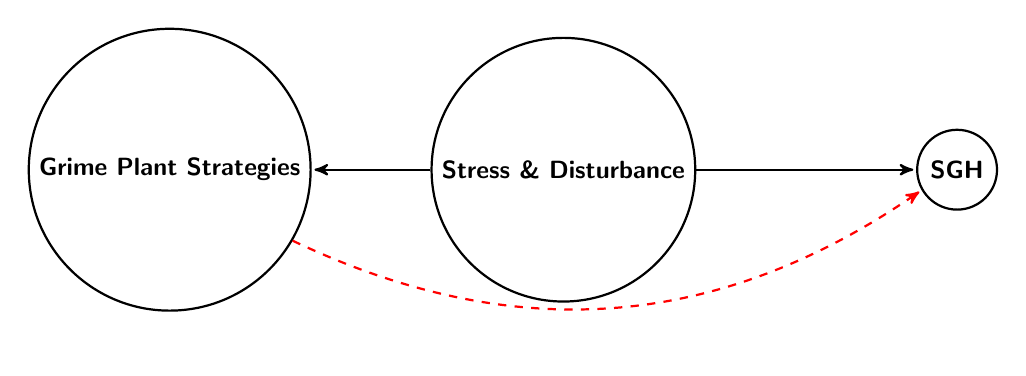
\begin{tikzpicture}[->,>=stealth',shorten >=1pt,auto,node distance=5cm,
                    thick,main node/.style={circle,draw,font=\sffamily\small\bfseries}]

  \node[main node] (1)  {Stress \& Disturbance};
  \node[main node] (2) [right of=1] { SGH };
  \node[main node] (3) [left of=1] {Grime Plant Strategies};

  \path[every node/.style={font=\sffamily\small}]
    (1) edge  node[right] {} (2)
    (1) edge  node {} (3)
    (3) edge [bend right,red, dashed] node  {} (2);
\end{tikzpicture}
\end{center}
\caption{In black: existing links in litterature. In red: Target link to add.}
\end{figure}


\begin{figure}
\begin{center}
\includegraphics[width=0.5\textwidth]{grime_english.pdf}
\end{center}
\caption{Diagram of Grime plant strategies along a gradient of Stress and disturbance.\label{Grime}}
\end{figure}



The goal of this studies is to have a functional approach of interaction inside a plant community in front of stress and disturbance gradient. We want to study how the interaction balance change along a stress and disturbance gradient at community level. To achieve this objective, we set up an experiment in South-East of Spain.

%%conceptual link between Grime and SGH model: (i) Facilitation can modulate Grime predictions ? (ii) Which strategies is the most facilitated along a stress and disturbance gradient ?

\part{Methods}

\section{Site}

The experiment will take in Alicante. Mart's field sites are free to use and those sites seem perfect. 3 independant terraces with each 2 plots: one is totally fenced to prevent grazing and one prevent grazing only from ruminant (rabbit can go in). 

\section{Plants}

It seems difficult to me to find caricatural species of grime's strategies but we can use instead species already used in experimental studies located in Mediteranean area. I used studies and reviews of \citet{McCluney2012,Navarro2006, Jauffret2003}.



\section{Design}

We have 3 plant species. I purposed a set of species to Susana and we have to see which can be used. We have 4 treatments: open/patch, grazing, water, alone/community and 3 blocks (terraces).

 We will simulate grazing instead of use goat. It will permit us to scale statistical unit to micro-site instead of plot as in previous experiment. We will simulate grazing by using probability of being eaten and how much thank to Mart's data. 
We will have a water-stress treatment provided by Susana's roof which exclude a bit less than 30\% of rainfall or if the summer is very dry, we can watering instead of exclude to have the water treatment.

For each terrace, we planted 30 saplings by treatment. Nurse micro-sites were choosen randomly and the corresponding open micro-site have been placed Xm around. Each species have been plant alone and in mix with the 2 other species. We performed  5 replicates for single species and the same for mix. So we need $10\times5\times3=150$ saplings of each species.


\begin{figure}
\begin{center}
\includegraphics[width=0.75\textwidth]{Experiment.pdf}
\end{center}
\caption{Resume of choosen treatment. Circle: adults; Square: saplings. Saplings are planted in triangular way and position is random in the triangle. Triangle are choosen to be sure saplings are at the same distance of main stem of the nurse. \label{exp}}
\end{figure}

Table \ref{hyp} shows assumptions about results of winning strategies according to stress or disturbance. In Summary, (i) we can think facilitation modulate Grime's prediction, (ii) we also make hypothesis that different strategies have different potential to be facilited.


\begin{table}
\begin{center}
\begin{tabular}{|l|l|l|l|l|l|}
  \hline
  & Control & Water stress & Low grazing & High grazing  \\
  \hline
  Patch & C & C & C & R \\
  \hline
  Open & C & S & S ou R & R \\
  \hline
\end{tabular} 
\end{center}
\caption{Hypothesis about winning plant strategies according to stress or disturbance.  Strategies: C (Competitive), R (Ruderal), S (Stress-tolerator). \label{hyp}}
\end{table}

\section{Measurements}
It would be good to measure height canopy and survival regularly to have dynamics of competition. Finally, the final output of competition would be an idea of seed production.


\section{Timing}
\begin{itemize}

\item End January: Drill hole.
\item February: plant saplings, watering them to prevent transplant mortality.
\item March: .
\item June or july: may be one visit to make sure everything is fine and water plants.
\item October: first measure and after application of grazing and water treatment.
\item March: Second measurement

\end{itemize}

%\bibliographystyle{plainnat}

%\bibliography{/home/alain.danet/Dropbox/Shared_TheseAlain/BibTeX/M2-StageM2,/home/alain.danet/Dropbox/Shared_TheseAlain/BibTeX/Thesis}
\printbibliography
\end{document}
\documentclass[12pt]{article} %scrartcl

%accents, language français
\usepackage[utf8]{inputenc}
\usepackage[T1]{fontenc}

% Outils graphiques
\usepackage{graphicx}
\usepackage{lscape}

\begin{document}

\begin{landscape}

\begin{center}
%\resizebox{\textwidth}{!} {
%{ \footnotesize % Réduire la taille de la police du tableau
\begin{tabular}{ccccc}
\hline 
Loose & Grazing tolerant & Grazing sensitive & Stress-tolerant & Competitive \\ 
\hline 
Teucrium polium & Fagonia cretica & Phlomis purpurea & \textit{Helianthemum squamatum} & \textit{Stipa tenacissima} \\ 

Koeleria vallesiana & Paronichia sufruticosa & Cistus albidus & \textit{Pistacia lentiscus} & \textit{Ligeum spartum} \\ 

Thymus lacaitae & Thymus & Quercus coccifera  & \textit{Lepidium subulatum} &  \\ 

Herniaria fruticosa & Teucrium & Olea europaea & \textit{Retama sphaerocarpa} &  \\ 

 & Sideritis spp. &  &  &  \\ 

 & A. herba-alba &  &  &  \\ 
\hline
\end{tabular} 
%}
%}
\end{center}
\end{landscape}

\end{document}
